\documentclass[]{article}

\usepackage{amsmath}
\usepackage{xcolor}
\usepackage{float}
\usepackage{graphicx}
\usepackage{authblk} % authors
\usepackage{booktabs} % pretty tables

% Supplementary Materials
\newcommand{\beginsupplement}{
	\setcounter{table}{0}
	\renewcommand{\thetable}{S\arabic{table}}
	\setcounter{figure}{0}
	\renewcommand{\thefigure}{S\arabic{figure}}
}

\title{Estimating my insulin-to-glucose ratios in preparation for flexible insulin therapy as a patient with type 1 diabetes}

\author{Rapha\"{e}l Scherrer}

\date{}

\begin{document}

\maketitle

\begin{abstract}
	
Self-management of type 1 diabetes can be constraining.
One approach to alleviate those constraints is flexible insulin therapy, where a patient picks a dose of insulin based on how much carbohydrates they eat, rather than the more traditional approach of adapting meals to fixed, pre-decided amounts of insulin.
In order to implement flexible insulin therapy, however, the right ratios must be known, for that patient, of insulin injected per gram of glucose consumed.
This requires extensive data on changes in blood sugar, or glycemia, in response to various amounts of carbohydrates eaten and insulin injected.
Here, I aimed at performing this analysis on myself, as a patient with type 1 diabetes.
Using recorded data over a span of two months and equipped with a continuous glucose monitoring system (CGM), I compiled a dataset comprising instances of food eaten, glycemia checked and insulin injected.
I also considered additional factors known to affect blood sugar such as physical activity, alcohol use and infections.
Unfortunately, the regression analyses performed did not result in parameter estimates that I could trust, probably due to mistakes in estimations of carbohydrate contents but also messy everyday life as opposed to if I had collected data in more controlled conditions.
Anyway, that was an insightful exercise which I thought to write up as to not forget how I did it.

\end{abstract}

\paragraph{Keywords} glycemia, carbohydrates, sugar, continuous glucose monitoring (CGM), diabetes self-management

\pagebreak

\section*{Introduction}

Managing blood sugar in type 1 diabetes can be challenging.
Already quite a lot of progress has been made for patients, thanks to continuous glucose monitoring (CGM) systems, for example, allowing a much more precise tracking of blood sugar levels than previous methods.
However, one challenge for any insulin-dependent diabetic patient is to know how much insulin to inject when eating something.
This is not trivial, as the right amount of insulin depends on the carbohydrates ingested, but also on confounding factors such as exercise, stress, alcohol and sickness (some of which, like alcohol and exercise, can have long-lasting effects).
It also changes from one person to another, as well as with age for a given person.\\

Usually, newly diagnosed patients are given a fixed amount of insulin to inject per meal, and are told how much carbs that amount of insulin corresponds to.
They then try to stick to that amount of carbohydrates at every meal, as much as possible.
It is possible to switch from that approach, where food is adapted to match the insulin injected, to a more flexible one where insulin can be adapted to accommodate the amount of food taken.
This latter approach is called flexible insulin therapy. 
Doing that, however, requires knowing precisely how much glucose can one's body absorb with a given amount of insulin, and that key variable must be measured on a case by case basis.\\

Here, I set out to do just that for myself.
To do that, I recorded basically everything happening in my life for a period of approximately two months, paying particular attention to amounts of carbohydrates eaten, insulin injected and physical activity.
Then, for each meal, or more broadly for each period after having eaten and being under the influence of insulin, I computed the observed change in glycemia over a certain period of time until blood sugar stabilization, and recorded the ratio of insulin injected per gram of ingested glucose over that period of time.
A regression analysis then allowed me to determine how much insulin I need to absorb a given amount of blood sugar, and given a certain desired change in glycemia.
Some additional steps were taken to include possible effects of activity, alcohol and sickness.
Unfortunately, the results did not seem reliable and so I did not end up using them, but I am still writing all this here, first, to remember how I did it, and second, in case it comes in useful some time in the future.

\pagebreak

\section*{Methods}

\subsection*{Data collection}

The data were collected over a period of approximately two months in the summer of 2024.
During that period, every glycemia measured, food intake, insulin injected and activity performed was recorded and timed.

\paragraph{Glycemia} Blood sugar was captured with continuous glucose monitoring (CGM) sensors FreeStyle Libre 2 (Abbott Laboratories, Chicago, Illinois, USA), changed every 14 days.
Glycemia was recorded in milligrams of glucose per deciliter of blood (mg/dL) with a FreeStyle Libre 2 reader version 1.2.2 1.03 (Abbott Laboratories).
For every glycemia read, I noted whether it was \textit{crashing}, \textit{decreasing}, \textit{stagnating}, \textit{increasing} or \textit{spiking} (as reported by the reader).
Glycemias that were too high (code ``HI'') or too low (code ``LO'') to be read by the reader were entered as \textit{non available}.

\paragraph{Food} Each food item (or drink) consumed was weighed and its carbohydrate content (in grams) calculated. 
The amount of carbohydrates was obtained from food packaging or from a general internet search.
Each food intake was also assigned a precision score based on the certainty of the assessment.
There, precisely measured foods scored as \textit{High}, foods of known weight but with approximately known sugar content (e.g. fruits) or the other way around (e.g. cooked rice or pasta when mixed with other things) scored as \textit{Medium}, and foods with both uncertain weight and uncertain content scored as \textit{Low}.

\paragraph{Insulin} Each injection of insulin was recorded in number of units.
The fast-acting insulin used was Humalog 100 units/mL (Lilly, Indianapolis, Indiana, USA). 
I also recorded when a fast insulin pen was over and started a new one.

\paragraph{Slow insulin} The slow-acting insulin was Tresiba 100 units/mL (Novo Nordisk, Bagsværd, Denmark). 
I recorded each injection, and since the effect of  this insulin lasts for more than 24 hours, I recorded for each event whether I was under its influence if the last slow insulin was injected 25 hours before or less.

\paragraph{Alcohol} I also estimated the alcohol content of each food and used it to assign a (subjective) inebriation status for each alcoholic beverage ingested.
This status could take the values 0 (no alcohol), 1 (some alcohol taken but sober), 2 (more than a drink but not yet tipsy), 3 (tipsy) and 4 (drunk, not reached within the recorded data).

\paragraph{Activity} Physical activity was recorded in terms of time, type of activity and intensity (\textit{Light}, \textit{Moderate} or \textit{Intense}).
However, I noticed that physical intensity is a poor predictor of how exercise affects blood sugar, with the most intense activities such as calisthenics workouts barely affecting glycemia, and more stamina-based activities such as walking, biking or running affecting it much more.
Therefore, I assigned an activity impact score to each recorded instance of physical exercise, based on my (subjective) perception of how impactful the activity is for my blood sugar.
The possible values were 0 (no effect, e.g. workout or doing the dishes), 1 (quite negligible effect, e.g. walk or bike up to 15min, or cooking for up to 60min), 2 (moderate effect that requires precaution, in that I may have to eat something afterwards, e.g. walk between 15 and 60min, bike between 15 and 30min, cleaning chores of 30min or more), 3 (taxing effect, will have to eat unless very high in glycemia already, e.g. walk of 60min or more, bike of 30min or more) and 4 (very taxing, never to be done without sugar on me, e.g. running 45min or more).

\paragraph{Sickness} Finally, I recorded whether I was sick or not during each of the aforementioned recorded events.

\paragraph{Missing data} Some periods of time were not recorded and entered as \textit{Missing}.
Other times, missing information in otherwise recorded events (e.g. missing carbohydrate content) was entered as \textit{non available}.

\subsection*{Processing}

I used the recorded database to identify (semi-)independent chunks of time, each to be used as data points in an analysis of how much a given amount of insulin affects glycemia, for a given amount of carbohydrates.
Those stable chunks of time were identified as time spans between any two consecutive ``key'' glycemias.
Glycemias were considered key glycemias when they were stable (recorded as \textit{stagnating} by the reader) and measured more than 1h30min, 2h ($\pm10$min) or 3h ($\pm 15$min) after the last insulin injection or food intake.
These time thresholds were chosen to ensure that a given chunk of time was no longer under the influence of food or insulin from a previous period (so the higher the time threshold, the lower the influence but the lower the number of data points available).
The analysis was repeated with each of these three time thresholds separately.
Chunks of time containing \textit{Missing} events were discarded, and food or insulin taken 5min or less before the beginning of a chunk were not taken as influencing that chunk (not enough time to affect blood sugar).
\textcolor{red}{So I should count them as part of the chunk in the analysis.}\\

I then summarized relevant variables on a per-chunk basis.
For each given time threshold ($1.5$, $2$ and $3$ hours), I extracted, for each identified chunk of time, (1) the starting time, (2) the end time, (3) stable blood sugar (i.e. ``key'' glycemia) at the starting time, (4) stable blood sugar at the end time, (5) the total amount of insulin injected during that time, (6) the total amount of carbohydrate ingested, (7) whether any of the carbohydrate content measured in that time was with low precision, (8) whether all of the time was spent under slow insulin, (9) whether the maximum inebriation status during that time was 2 or more (more than a drink was consumed), (10) whether the cumulative impact score of all physical activity during that time was 2 or more (the equivalent of more than two walks of 15min), (11) whether the time chunk was particularly long (more than 500min) and (12) whether I was sick at the start of the chunk.\\

As a final step, I computed the ratio of insulin injected to glucose consumed (in units/g), and the observed change in glycemia (in mg/dL) for each chunk.
The change in glycemia was then scaled by the amount of glucose consumed.
This is because the change in glycemia is proportional to the amount of glucose left over in the blood (and not assimilated by the injected insulin) and not to the insulin-to-glucose ratio (e.g. enough insulin to assimilate half of the glucose in a food item will still leave twice as much glucose surplus in the blood when eating twice as much of that food item).
This glucose surplus, in turn, is equal to the total amount of glucose ingested minus the amount absorbed, which is itself a proportion of the total glucose that is proportional to the insulin-to-glucose ratio.
Hence, the change in glycemia $\Delta g$ can be written as

\begin{equation}
    \Delta g = \beta \, (G - \alpha \, I)
    \label{eq:delta_g}
\end{equation}

\noindent where $G$ is the total amount of glucose, $I$ is the total amount of insulin injected, $\beta$ is the conversion constant of glucose surplus into a change in glycemia, and $\alpha$ is a conversion constant of insulin-to-glucose ratio into a proportion of glucose absorbed.
It follows, in turn, that both $G$ and $I$ must be known to predict $\Delta g$, but that the ``re-scaled'' change in glycemia, $\Delta g / G$ can be known from knowing the insulin-to-glucose ratio $I / G$ alone.
In what follows, I analyze statistically the effect of the insulin-to-glucose ratio on the scaled change in glycemia.\\ 

Eyeballing the results (Fig. \ref{fig:overview}), I found that there were not many chunks with imprecise data or where I was not under slow insulin, for any of the time thresholds.
For the subsequent analysis, I therefore only kept data points with medium-to-high precision, and fully covered by slow insulin, as this did not incur much data loss.
Besides, chunks where some insulin was injected but no glucose were discarded, as they resulted in infinite insulin-to-glucose ratios.
\textcolor{red}{Could analyze those alone though.}
Finally, I discarded outliers, visually considered as having an insulin-to-glucose ratio greater than $0.4$.

\subsection*{Analysis}

I analyzed the data by performing a linear regression of the scaled change in glycemia against the ratio of insulin to glucose.
Based on previous knowledge on what affects blood sugar I decided to treat activity, alcohol and sickness as (binary) confounding variables.
As I did not notice any particular pattern with respect to insulin cartridge and whether chunks were very long (Fig. \ref{fig:overview}), I did not consider those two variables in the analysis.
Besides, as the different combinations of activity, alcohol and sickness status were very uneven in numbers of observations (not shown), I decided not to include interaction effects between any of those confounding variables.\\

In addition, a regression analysis with one regression line for each combination of activity, alcohol and sickness, resulted in odd slopes and seemed to suffer much from the reduction in degrees of freedom (not shown).
\textcolor{red}{But it actually looks fine for 3 hours, so try with that?.}
I therefore decided not to trust this analysis and instead fit four different models: (1) a general regression of scaled change in glycemia against insulin-to-glucose ratio, (2) same but with two regressions split by activity, (3) by alcohol and (4) by sickness (see e.g. Fig. \ref{fig:regressions}).
I then extracted the regression parameters (slopes and intercepts) of the model with no confounder as representative of the ``normal'' state (no activity, no alcohol and not sick), and of the lines corresponding to activity, alcohol and sickness, in the three remaining respective models (Table \ref{tab:parameters}, with parameters $\alpha$ and $\beta$ inferred from equating the regression line equation of $\Delta g / G$ against $I / G$ to Equation \ref{eq:delta_g}).

\subsection*{Predictions}

I used the calculated parameters to predict the amount of insulin needed for any given amount of carbohydrate ingested and targeted change in glycemia.
Depending on the state (activity, alcohol, sickness) and based on a certain time threshold (Table \ref{tab:parameters}), the formula to do that is

\begin{equation}
    I = \big(\Delta g - \text{intercept} * G\big) / \text{slope} \; ,
\end{equation}

\noindent in units of insulin.


\pagebreak

\section*{Results}

The results are best shown in an ``injection table'' giving the amount of insulin to inject (in units) for a given glucose intake (in grams) and for a given desired change in glycemia (in mg/dL).
Table \ref{tab:injections} shows one such table for the ``normal'' state (average across activity, alcohol and sickness status) for a time threshold of 3 hours.
\textcolor{red}{Should I not distinguish ``normal'' and ``average'' then?}\\

It seemed that a time threshold of three hours gave the most reliable results, and so I only show those in Fig. \ref{fig:regressions} and Table \ref{tab:injections}.
Still, the predicted insulin injections were very odd, with (based on my own experience) very low doses for glucose intakes that I know should require more (e.g. $1.5$ units to increase glycemia by $50$ mg/dL when eating $65$ grams of glucose), and very high doses for other changes in glycemia which I know require much less insulin (e.g. $17.6$ units to decrease glycemia by $300$ mg/dL when eating nothing, Table \ref{tab:injections}). 
And so, although the exercise was valuable, I decide not to trust those results.

\pagebreak

\section*{Discussion}

There are several reasons why the results are not trustworthy.
First, the data were collected in everyday life, so non-control conditions, with lots of confounding factors known to have an effect on blood sugar (exercise, stress, etc.).
Second, because of the non-control conditions, the chunks of time taken as data points were of varying durations, with some chunks spanning multiple meals and multiple activities until blood sugar stabilizes.
The increase in cumulative insulin and cumulative glucose (and exercise when applicable) during those periods may have introduced imprecisions in the data.
Third, there probably were mistakes in the estimation of the actual carbohydrates taken in, whether due to imprecise weighing or incorrect carbohydrate contents of the food items.\\

The solution seems to be to repeat this kind of analysis in controlled conditioned, that is, with much less variation in time span, and by removing as many confounding factors as possible.
Of course, this may affect the generality of the results regarding everyday life, but at least would provide a solid and reliable baseline for how much insulin is needed to absorb a given amount of sugar.
Those doses could then be slightly modified when under stress, alcohol, sick or when doing exercise.
That said, I noticed that the breakfast recorded in the data were especially consistent and precise, resembling controlled conditions.
\textcolor{red}{Maybe I could repeat my analysis on the same data but only looking at those and see if the predictions are more reliable.}


\pagebreak

\section*{Tables}

\begin{table}[H]
	\caption{Estimated parameter values for different time thresholds. $\beta$, conversion parameter of glucose surplus into change in glycemia (equal to the intercept); $\alpha$, conversion constant insulin-to-glucose ratio into proportion of absorbed glucose (equal to minus the slope divided by the intercept). See Methods for details.}
	\centering
	
\begin{tabular}{lrrrrr}
\toprule
State & Intercept & Slope & $\beta$ & $\alpha$ & Threshold (hours)\\
\midrule
Normal & 0.557 & -5.906 & 0.557 & 10.597 & 1.5\\
Activity & 0.650 & -3.737 & 0.650 & 5.754 & 1.5\\
Alcohol & 0.648 & -9.387 & 0.648 & 14.496 & 1.5\\
Sick & 1.235 & -16.343 & 1.235 & 13.228 & 1.5\\
\addlinespace
Normal & 0.509 & -6.621 & 0.509 & 13.006 & 2.0\\
Activity & 0.471 & -2.125 & 0.471 & 4.508 & 2.0\\
Alcohol & 0.192 & -4.441 & 0.192 & 23.121 & 2.0\\
Sick & 1.130 & -16.971 & 1.130 & 15.015 & 2.0\\
\addlinespace
Normal & 1.094 & -17.038 & 1.094 & 15.573 & 3.0\\
Activity & 1.435 & -18.561 & 1.435 & 12.938 & 3.0\\
Alcohol & 1.048 & -14.270 & 1.048 & 13.618 & 3.0\\
Sick & 0.929 & -12.752 & 0.929 & 13.729 & 3.0\\
\bottomrule
\end{tabular}
	\label{tab:parameters}
\end{table}

\pagebreak

\begin{table}[H]
	\caption{Injection table showing how many units of insulin to inject for a given glucose intake (left column, in grams) and desired change in glycemia (top row, in mg/dL). Those results are based on parameter estimates for the ``normal'' state and a time threshold of 3 hours (see Table \ref{tab:parameters}). NA, not available.}
	\centering
	
\begin{tabular}{rrrrrrrrrrrrrr}
\toprule
Glucose & -300 & -250 & -200 & -150 & -100 & -50 & 0 & 50 & 100 & 150 & 200 & 250 & 300\\
\midrule
0 & 17.6 & 14.7 & 11.7 & 8.8 & 5.9 & 2.9 & 0.0 & NA & NA & NA & NA & NA & NA\\
5 & 17.9 & 15.0 & 12.1 & 9.1 & 6.2 & 3.3 & 0.3 & NA & NA & NA & NA & NA & NA\\
10 & 18.3 & 15.3 & 12.4 & 9.4 & 6.5 & 3.6 & 0.6 & NA & NA & NA & NA & NA & NA\\
15 & 18.6 & 15.6 & 12.7 & 9.8 & 6.8 & 3.9 & 1.0 & NA & NA & NA & NA & NA & NA\\
20 & 18.9 & 16.0 & 13.0 & 10.1 & 7.2 & 4.2 & 1.3 & NA & NA & NA & NA & NA & NA\\
25 & 19.2 & 16.3 & 13.3 & 10.4 & 7.5 & 4.5 & 1.6 & NA & NA & NA & NA & NA & NA\\
30 & 19.5 & 16.6 & 13.7 & 10.7 & 7.8 & 4.9 & 1.9 & NA & NA & NA & NA & NA & NA\\
35 & 19.9 & 16.9 & 14.0 & 11.1 & 8.1 & 5.2 & 2.2 & NA & NA & NA & NA & NA & NA\\
40 & 20.2 & 17.2 & 14.3 & 11.4 & 8.4 & 5.5 & 2.6 & NA & NA & NA & NA & NA & NA\\
45 & 20.5 & 17.6 & 14.6 & 11.7 & 8.8 & 5.8 & 2.9 & NA & NA & NA & NA & NA & NA\\
50 & 20.8 & 17.9 & 14.9 & 12.0 & 9.1 & 6.1 & 3.2 & 0.3 & NA & NA & NA & NA & NA\\
55 & 21.1 & 18.2 & 15.3 & 12.3 & 9.4 & 6.5 & 3.5 & 0.6 & NA & NA & NA & NA & NA\\
60 & 21.5 & 18.5 & 15.6 & 12.7 & 9.7 & 6.8 & 3.9 & 0.9 & NA & NA & NA & NA & NA\\
65 & 21.8 & 18.8 & 15.9 & 13.0 & 10.0 & 7.1 & 4.2 & 1.2 & NA & NA & NA & NA & NA\\
70 & 22.1 & 19.2 & 16.2 & 13.3 & 10.4 & 7.4 & 4.5 & 1.6 & NA & NA & NA & NA & NA\\
75 & 22.4 & 19.5 & 16.6 & 13.6 & 10.7 & 7.8 & 4.8 & 1.9 & NA & NA & NA & NA & NA\\
80 & 22.7 & 19.8 & 16.9 & 13.9 & 11.0 & 8.1 & 5.1 & 2.2 & NA & NA & NA & NA & NA\\
85 & 23.1 & 20.1 & 17.2 & 14.3 & 11.3 & 8.4 & 5.5 & 2.5 & NA & NA & NA & NA & NA\\
90 & 23.4 & 20.5 & 17.5 & 14.6 & 11.6 & 8.7 & 5.8 & 2.8 & NA & NA & NA & NA & NA\\
95 & 23.7 & 20.8 & 17.8 & 14.9 & 12.0 & 9.0 & 6.1 & 3.2 & 0.2 & NA & NA & NA & NA\\
100 & 24.0 & 21.1 & 18.2 & 15.2 & 12.3 & 9.4 & 6.4 & 3.5 & 0.6 & NA & NA & NA & NA\\
\bottomrule
\end{tabular}
	\label{tab:injections}
\end{table}

\pagebreak

\section*{Figures}

\begin{figure}[H]
	\centering
	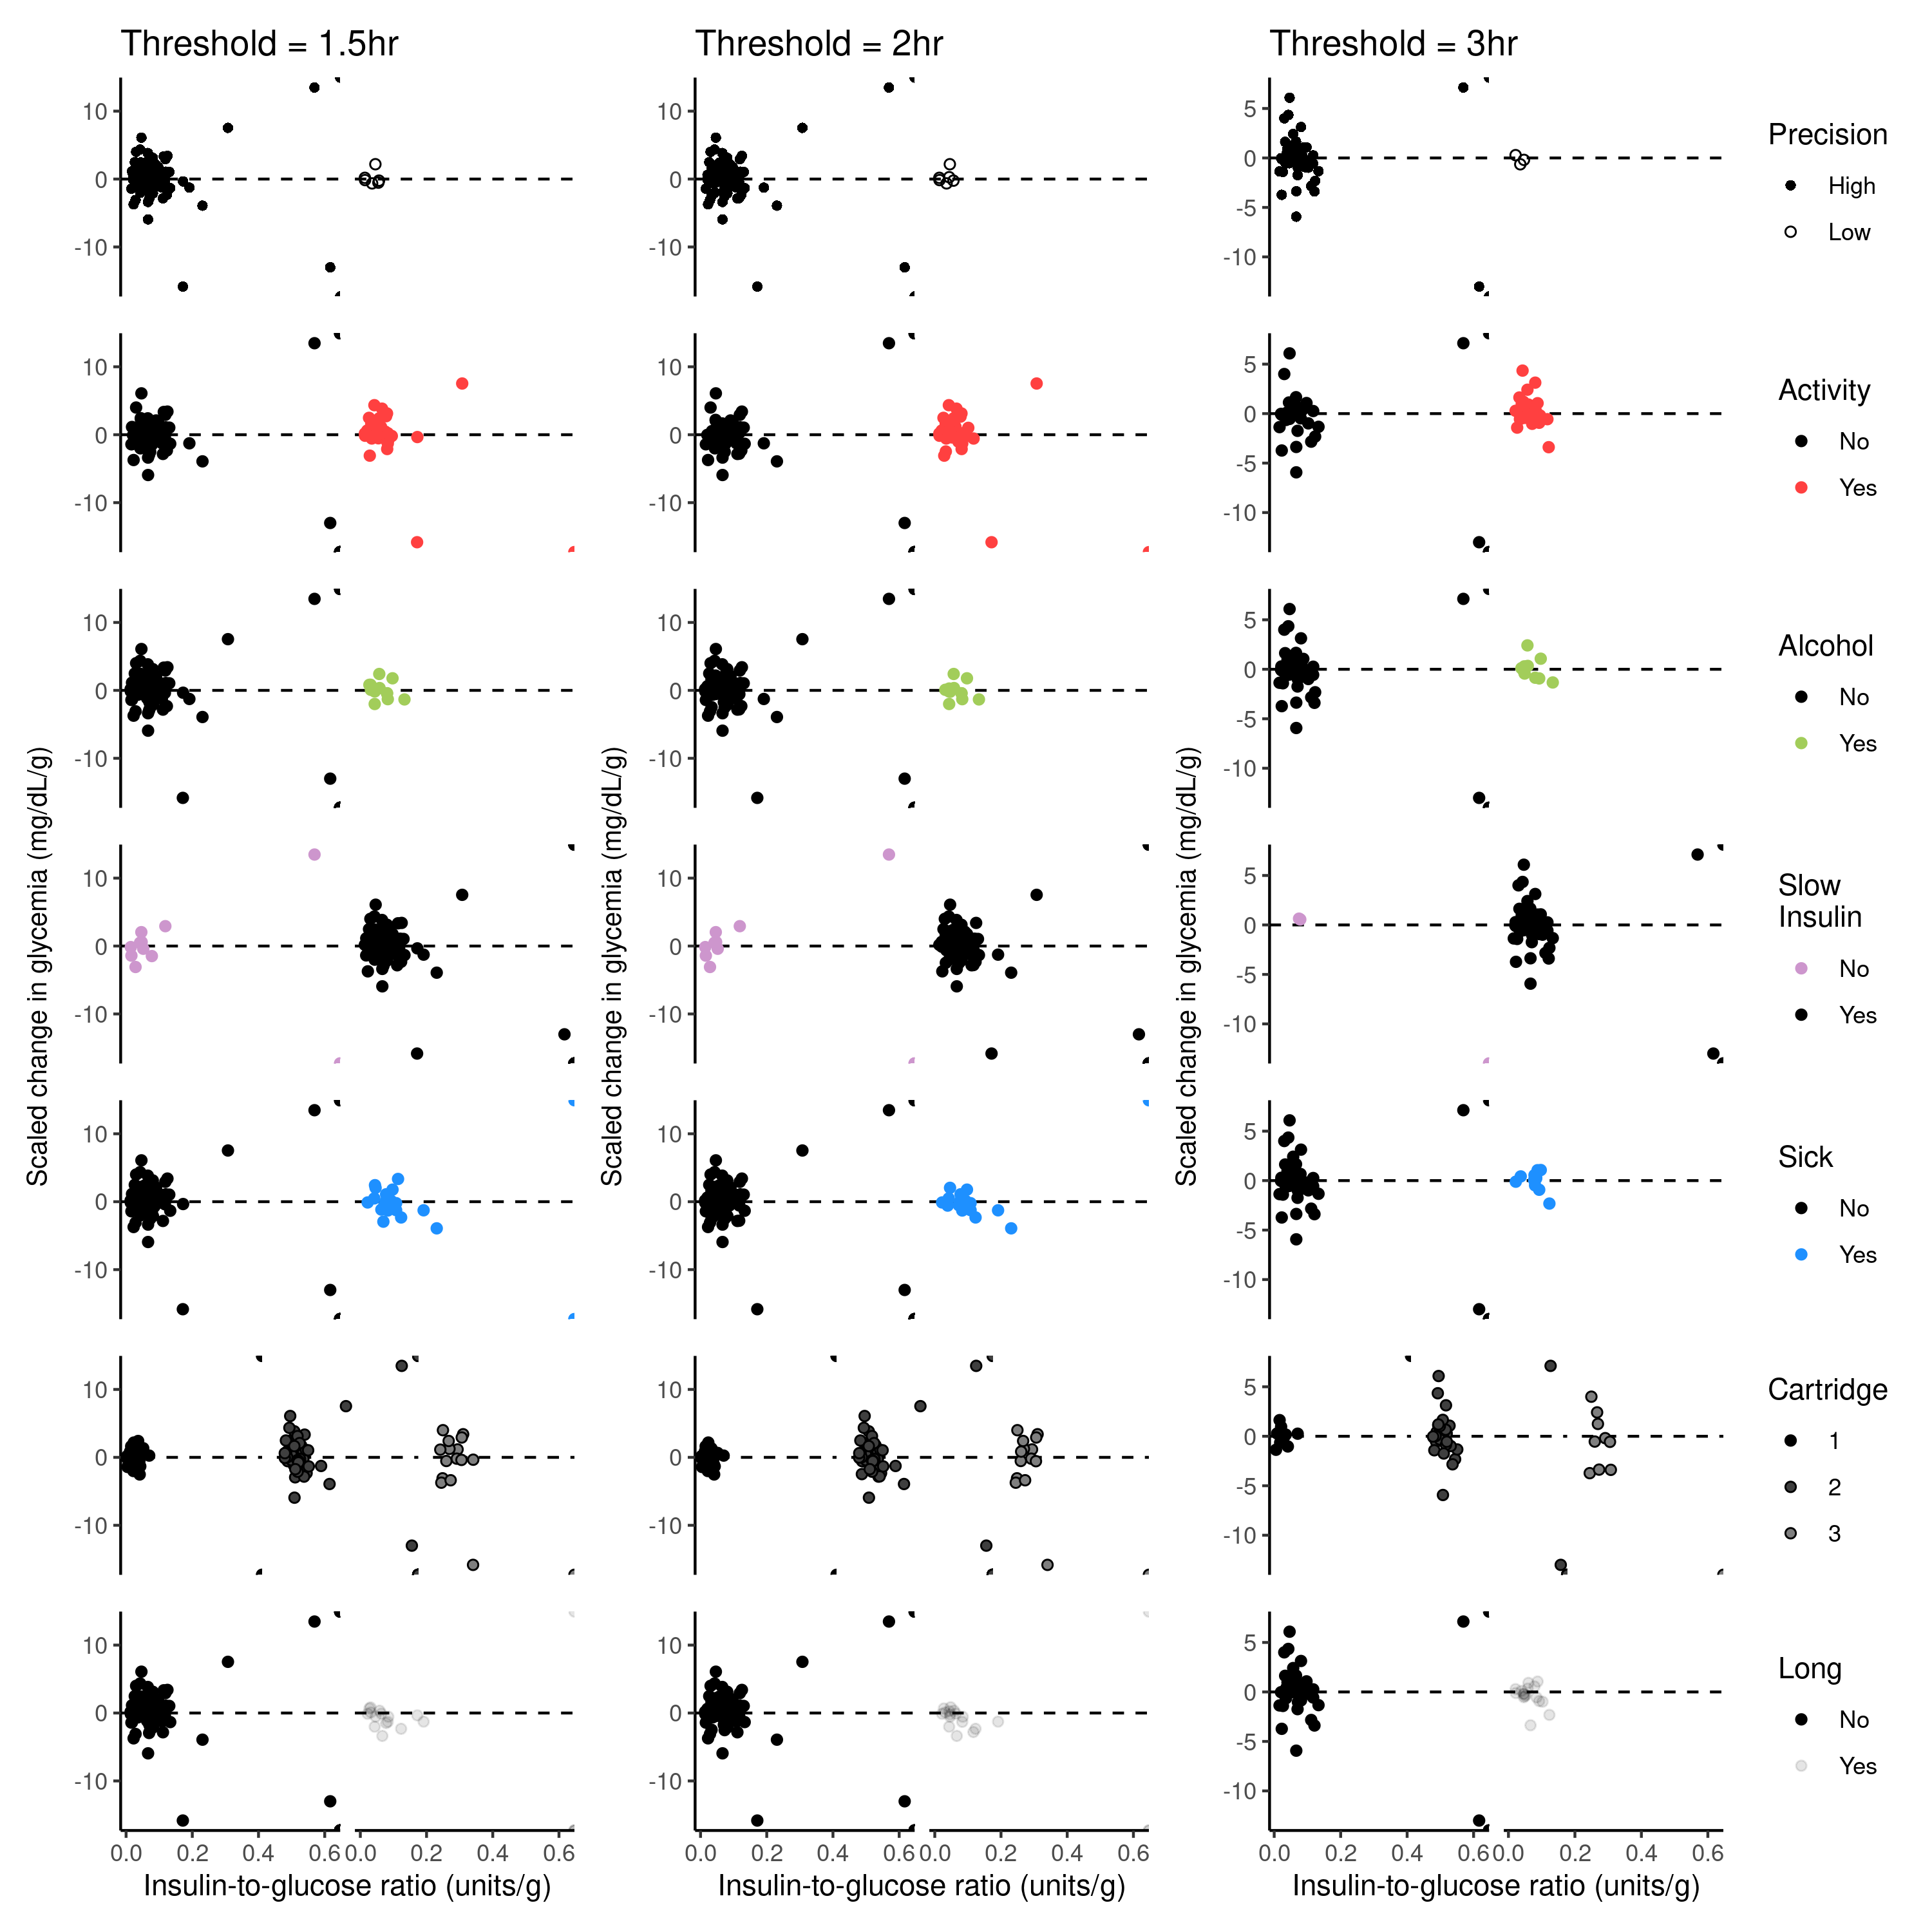
\includegraphics[width=\textwidth]{figures/overview_binary.png}
	\caption{Overview of the data split by various values of the confounding variables, and for three different time thresholds (see Methods). Precision, whether there was a low-precision glucose measurement; Activity, whether the total activity impact score was of 2 or more; Alcohol, whether the highest inebriation status was of 2 or more; Slow Insulin, whether slow insulin was having an effect; Cartridge, identifier for individual insulin cartridges; Long, whether the chunk was more than 500min long. Note the difference of scales when splitting by cartridge (because of three cartridges).}
	\label{fig:overview}
\end{figure}

\pagebreak

\begin{figure}[H]
	\centering
	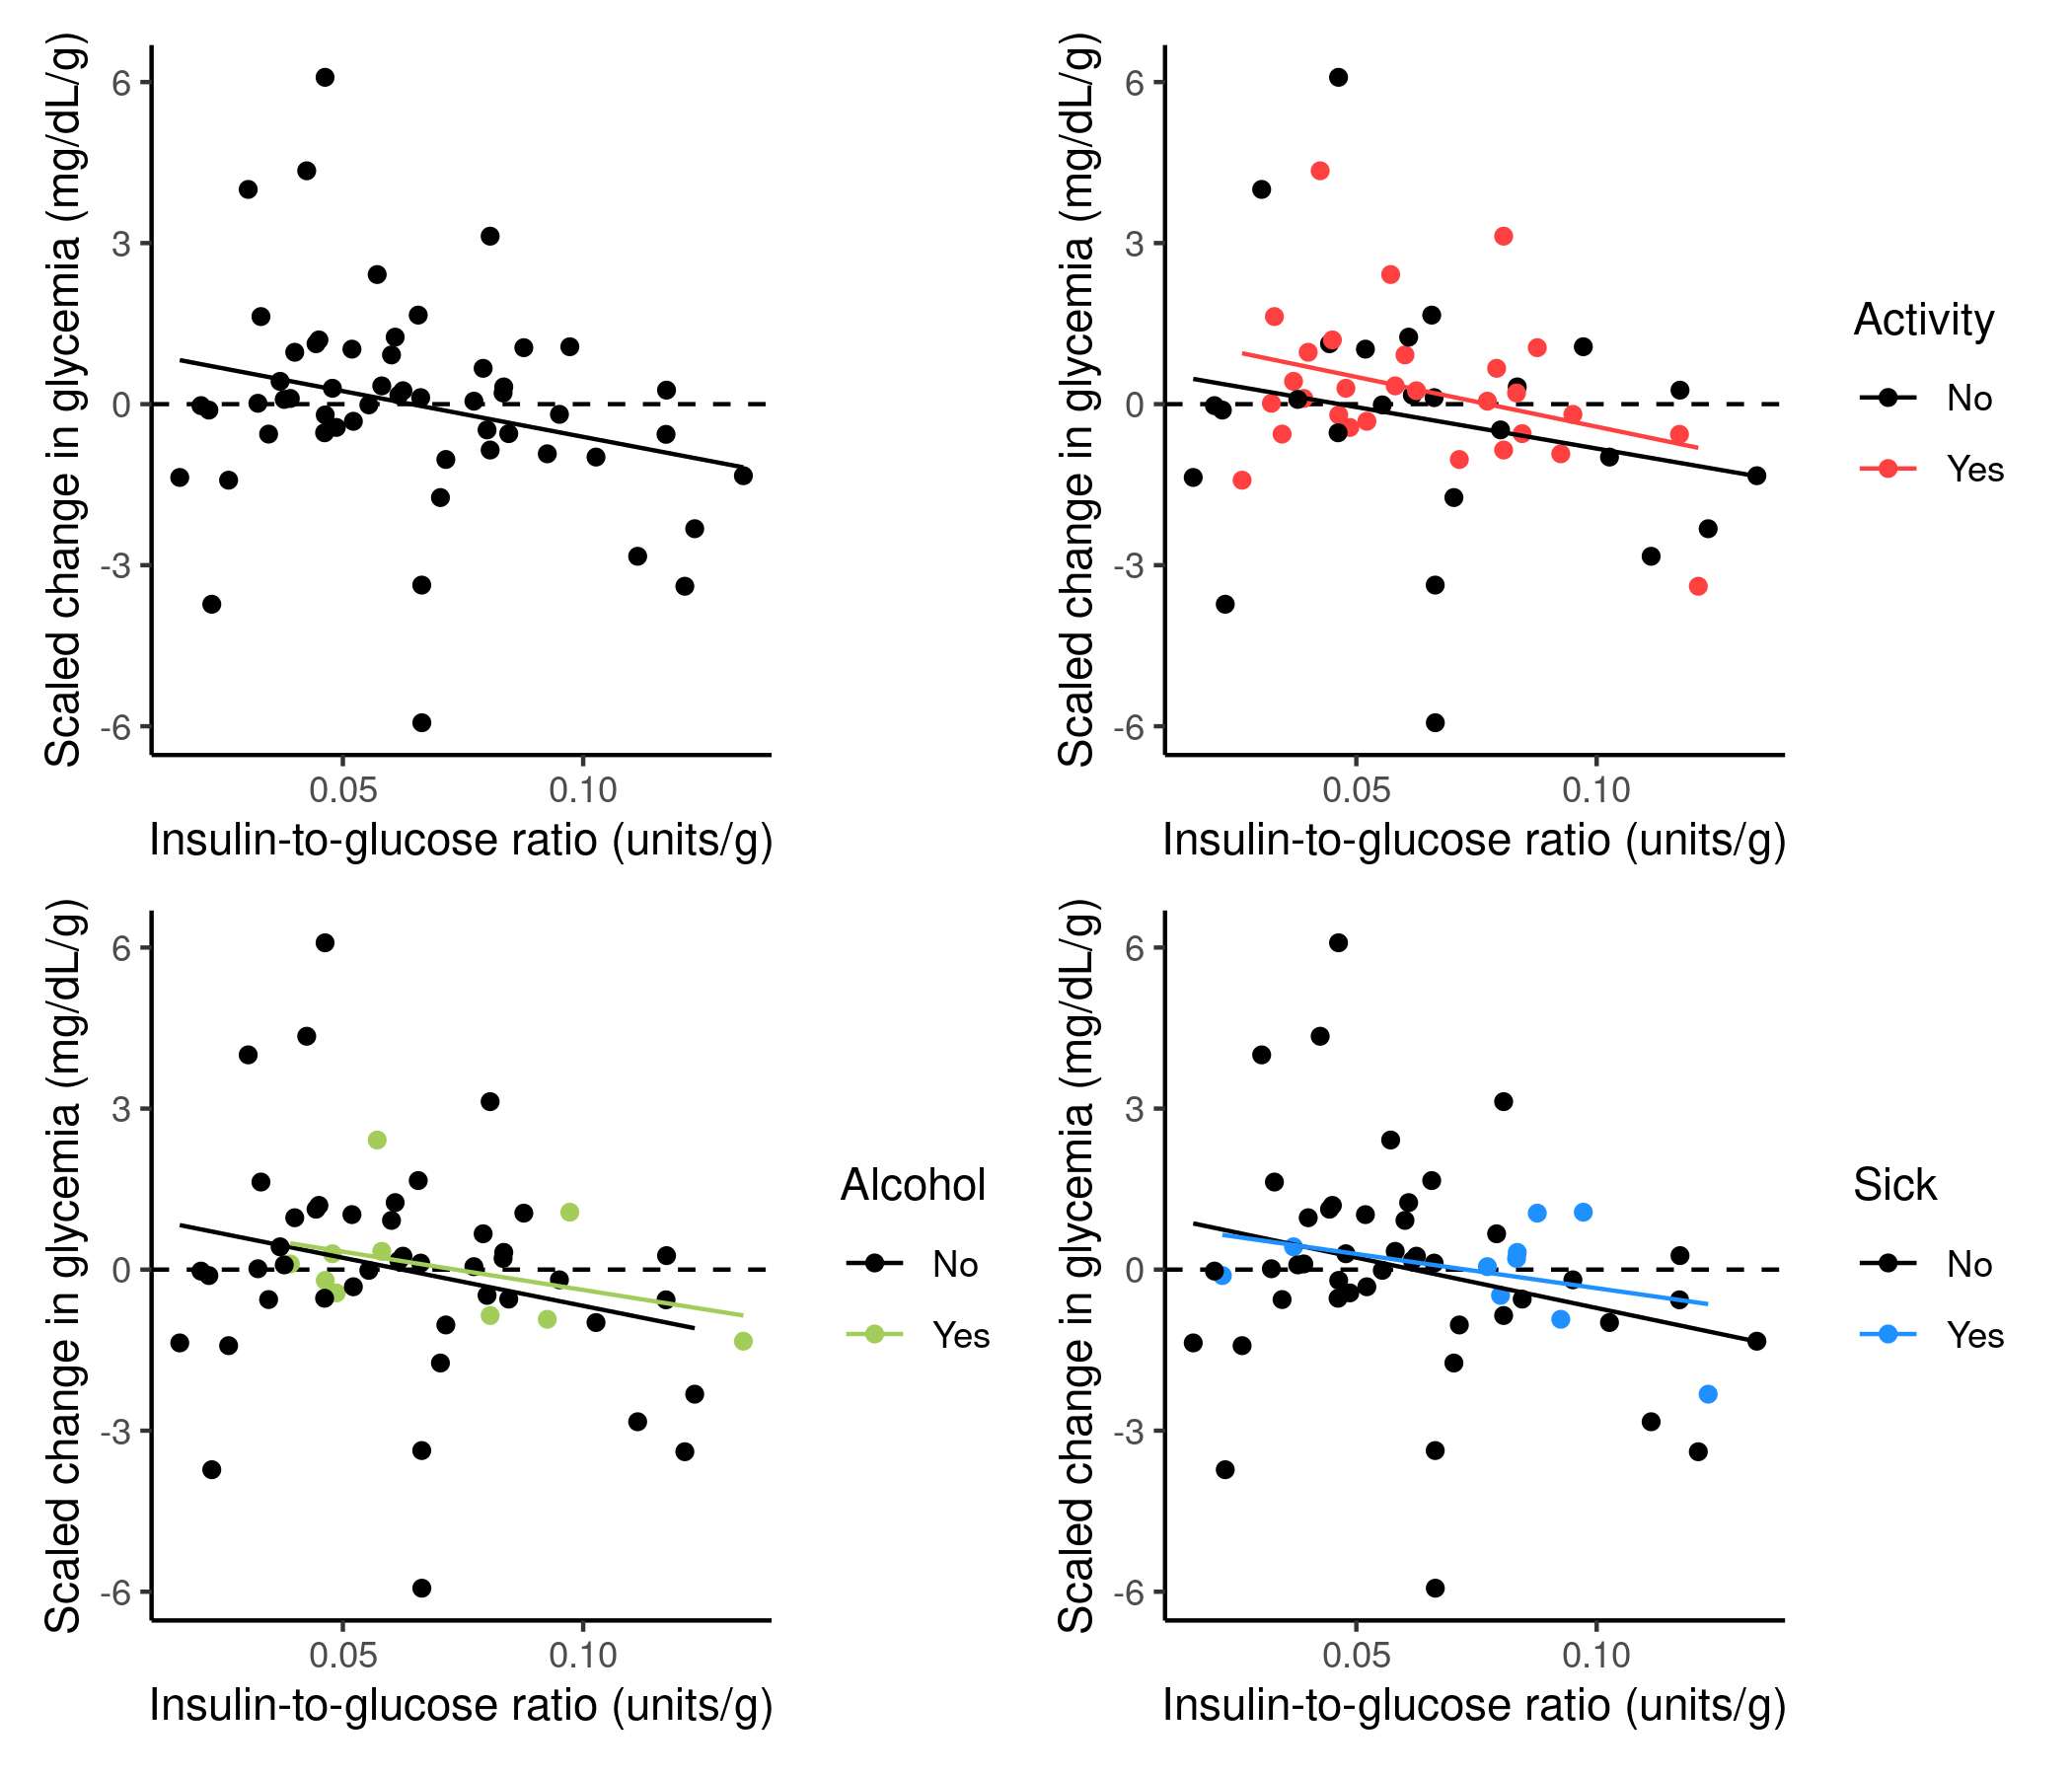
\includegraphics[width=\textwidth]{figures/separate_regressions_3_0.png}
	\caption{Four separate regression analyses of scaled change in glycemia against insulin-to-glucose ratio, either with no confounding variable (top left), or including activity (top right), alcohol (bottom left) or sickness (bottom right) as confounder. Those results are for a time threshold of 3 hours.}
	\label{fig:regressions}
\end{figure}

\end{document}
